Tato kapitola je věnována návrhu informačního systému pro správu třídních knih. V prvé řadě budou vytvořeny případy užití, tedy průchody budoucí aplikací. Ty představují návrh toho, jak bude systém naplňovat funkční požadavky, které byly definovány v předchozí kapitole určené analýze. Dále bude věnován prostor architektonickému návrhu systému. Zde bude zvolena vhodná architektura, která bude použita při implementaci aplikace. Poslední část kapitoly bude věnována návrhu uživatelského rozhraní několika základních obrazovek.

\section{Model případů užití}
Model případů užití slouží k detailní specifikaci funkčních požadavků. Navrhují se průchody budoucí aplikací. Typicky obsahuje seznam účastníků, diagram případů užití a jejich popis. Slouží jako zadání pro programátora, tvorbu akceptačních testů či tvorbě uživatelské příručky. \cite{pripady-uziti-prednaska}
\clearpage
\subsection{Účastníci}
Obrázek \ref{ucastnici} zobrazuje uživatele systému. Účastníci jsou použiti jako aktéři v případech užití.

\begin{figure}[h]
	\centering
	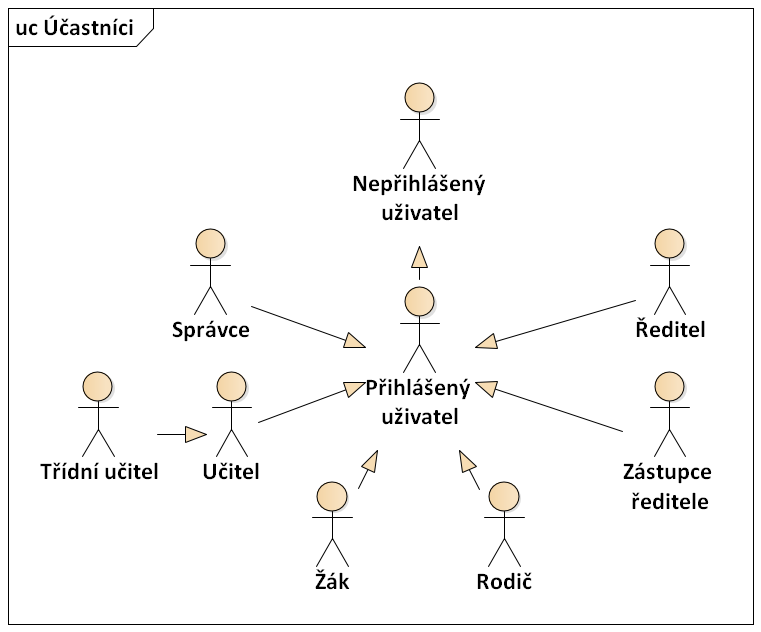
\includegraphics[width=\textwidth]{images/ucastnici.png}
	\caption{Aktéři případů užití}
	\label{ucastnici}
\end{figure}

\clearpage
\subsection{Případy užití}
\subsubsection{Obecné}
Na obrázku \ref{pripady-obecne} lze vidět namodelované obecné případy užití.

\begin{figure}[h]
	\centering
	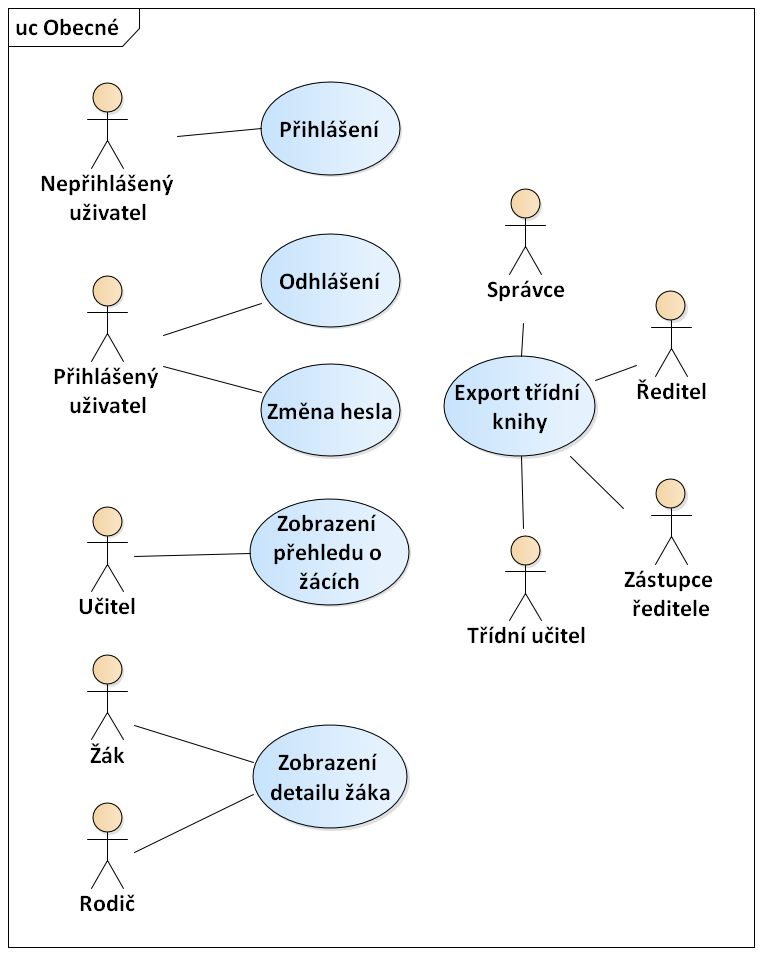
\includegraphics[width=\textwidth]{images/obecne.png}
	\caption{Obecné případy užití}
	\label{pripady-obecne}
\end{figure}

\subsubsection*{UC1 Přihlášení}
Umožňuje nepřihlášenému uživateli přihlášení do systému. 
\begin{itemize}
    \item Uživatel vyplní e-mail a heslo a klikne na tlačítko \uv{Přihlásit}, čímž se přihlásí do systému.
\end{itemize}

\subsubsection*{UC2 Změna hesla}
Umožňuje uživateli změnit přístupové heslo.
\paragraph{Hlavní scénář}
\begin{itemize}
    \item Uživatel se přihlásí do systému.
    \item Rozklikne ovládací menu a zvolí položku \uv{Účet}.
    \item Klikne na tlačítko pro změnu hesla.
    \item Dostane se na formulář pro změnu hesla, kde zadá stávající heslo, nové heslo a potvrzení nového hesla. Po potvrzení formuláře se heslo změní.
\end{itemize}

\paragraph{Alternativní scénář}
\begin{itemize}
    \item Nepřihlášený uživatel na přihlašovací obrazovce stiskne tlačítko pro zapomenuté heslo, čímž se dostane na formulář pro obnovu hesla.
    \item Ve formuláři zadá e-mailovou adresu, kterou se přihlašuje do systému.
    \item Na zadaný e-mail mu přijde odkaz, který ho přesměruje na formulář pro zadání nového hesla. 
    \item Ve formuláři vyplní nové heslo a potvrzení nového hesla. Po potvrzení formuláře se heslo změní.
\end{itemize}

\subsubsection*{UC3 Odhlášení}
Umožňuje odhlášení uživatele ze systému.

\subsubsection*{UC4 Export třídní knihy}
Umožňuje uživateli s rolí správce, ředitele, zástupce ředitele nebo třídního učitele vyexportovat třídní knihu do souboru PDF.
\begin{itemize}
    \item Uživatel s požadovanou rolí se přihlásí do systému.
    \item V navigačním menu si vybere políčko, které mu ukáže seznam třídních knih.
    \item U položky, která odkazuje na danou třídní knihu klikne na tlačítko pro export třídní knihy.
    \item Tím se dostane na formulář, kde zadá časový rozsah, ve kterém chce třídní knihu tisknout.
    \item Potvrzením formuláře vygeneruje systém PDF soubor s třídní knihou.
\end{itemize}

\subsubsection*{UC5 Zobrazení přehledu o žácích}
Umožňuje uživatelům s příslušnou rolí zobrazit si seznam žáků s jejich přehledem. Přehled si mohou zobrazit uživatelé s rolí učitel, ředitel, zástupce ředitele a správce.
\begin{itemize}
    \item Uživatel se přihlásí do systému.
    \item V navigačním menu se přepne do sekce s přehledy.
    \item Po výběru třídy z nabídky se uživateli zobrazí seznam žáků v dané třídě.
    \item U každého žáka v seznamu je možné přejít na jeho detail.
\end{itemize}

\subsubsection*{UC6 Zobrazení detailu žáka}
Umožňuje zobrazit informace o žákovi. Bude zobrazovat informace o absenci, poznámkách či domácích úkolech. Detail si může zobrazit samotný žák, jeho rodič, všichni učitelé, ředitel, zástupce ředitele a správci.


\subsubsection{Zápis hodiny, omluvenky}
Obrázek \ref{pripady-zapis} zobrazuje namodelované případy užití, které slouží pro zápis do třídní knihy a práci s omluvenkami.


\begin{figure}[h]
	\centering
	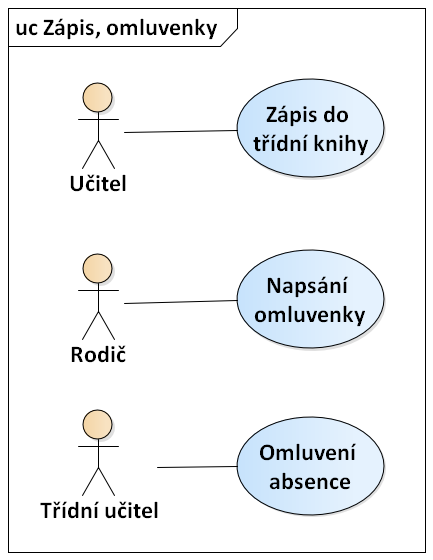
\includegraphics[width=0.5\textwidth]{images/zapis.png}
	\caption{Případy užití pro zápis a omluvenky}
	\label{pripady-zapis}
\end{figure}

\subsubsection*{UC7 Zápis do třídní knihy}
Umožňuje učiteli zapsat záznam o proběhnuté hodině do třídní knihy.
\begin{itemize}
    \item Učitel se přihlásí do systému.
    \item V navigačním menu si vybere políčko, které mu ukáže seznam třídních knih.
    \item Vybere si třídní knihu, do které chce zapsat.
    \item Tím se dostává na stránku, která zobrazuje záznamy v daném dni. Mezi dny lze přepínat.
    \item Stránka obsahuje tlačítko pro vytvoření nového záznamu. Po jeho stisknutí se dostává na formulář, kde může vytvořit nový zápis do třídní knihy.
    \item Ve formuláři vyplní předmět,  téma hodiny, případně číslo hodiny. Po potvrzení je vytvořen nový záznam v třídní knize. 
    \item Pro zadání absence žáků se použije tlačítko v řádku záznamu. 
    \item Po jeho stisknutí se učitel dostane na formulář, kde ze seznamu zaškrtne žáky, kteří nejsou přítomni, případně přišli pozdě.
    \item Potvrzením formuláře se aktualizují absence žáků.
\end{itemize}

\subsubsection*{UC8 Napsání omluvenky}
Umožňuje uživateli s rolí rodič napsat omluvenku, kterou omluví absenci svého potomka.
\begin{itemize}
    \item Rodič se přihlásí do systému.
    \item Přepne se do docházky a vybere potomka, kterého chce zobrazit.
    \item Zobrazí se seznam neomluvených absencí, ze kterých rodič vybere ty, které chce omluvit.
    \item Klikne na tlačítko pro napsání omluvenky.
    \item Dostane se na formulář, kde vyplní text omluvenky.
    \item Potvrzením formuláře omluvenku pošle třídnímu učiteli.
\end{itemize}

\subsubsection*{UC9 Omluvení absence}
Umožňuje třídnímu učiteli omluvit absenci žáka.
\paragraph{Hlavní scénář}
\begin{itemize}
    \item Třídní učitel se přihlásí do systému.
    \item V navigačním menu si vybere políčko pro zobrazení docházky.
    \item Na stránce vidí seznam omluvenek, které čekají na schválení.
    \item Třídní učitel může omluvenku potvrdit či zamítnout, případně si rozkliknout detail, který zobrazí, na které absence se omluvenka vztahuje.
\end{itemize}

\paragraph{Alternativní scénář}
\begin{itemize}
    \item Třídní učitel se přihlásí do systému.
    \item V navigačním menu si vybere políčko pro zobrazení docházky.
    \item Na stránce klikne na tlačítko pro zobrazení absencí žáků.
    \item Zde vidí seznam žáků, kteří mají neomluvené absence.
    \item Vybere žáka, u kterého chce omluvit absenci a klikne na tlačítko pro zobrazení detailu.
    \item Ze seznamu vybere, které absence chce omluvit.
    \item Klikne na tlačítko pro napsání omluvenky.
    \item Dostane se na formulář, kde vyplní text omluvenky a potvrdí.
\end{itemize}

\subsubsection{Události}
Na obrázku \ref{pripady-udalosti} lze vidět případy užití věnující se událostem v hodině.

\begin{figure}[h]
	\centering
	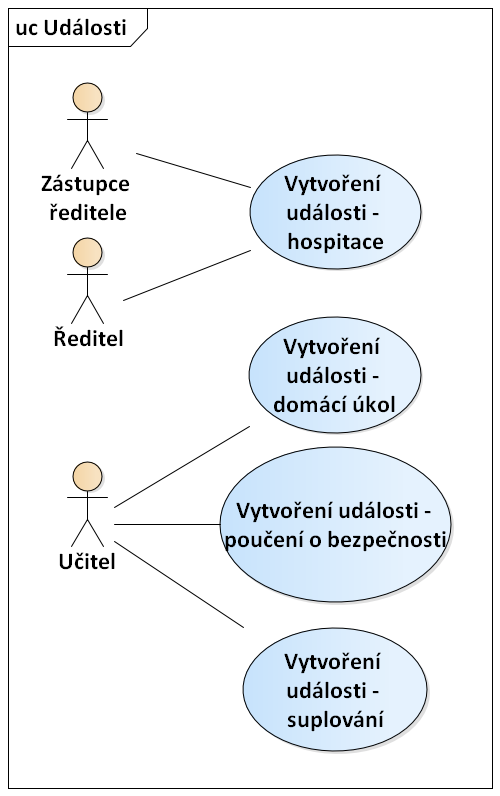
\includegraphics[width=0.6\textwidth]{images/udalosti.png}
	\caption{Případy užití pro události v hodině}
	\label{pripady-udalosti}
\end{figure}

\subsubsection*{UC10 Vytvoření události -- hospitace}
Umožňuje uživateli s rolí ředitel nebo zástupce ředitele přidat do třídní knihy informaci o proběhnuté hospitaci v hodině.

\begin{itemize}
    \item Uživatel s požadovanou rolí se přihlásí do systému.
    \item V navigačním menu se přepne do třídní knihy a vybere třídní knihu třídy, kde bude probíhat hospitace.
    \item Tím se dostává na stránku, která zobrazuje záznamy v daném dni.
    \item U požadované hodiny klikne na tlačítko pro zobrazení menu dalších akcí. 
    \item Ze seznamu vybere tlačítko pro přidání hospitace.
    \item Zobrazí se formulář, kde vyplní jméno hospitujícího a zápis z hospitace. Potvrzením formuláře je hospitace vytvořena.
\end{itemize}


\subsubsection*{UC11 Vytvoření události -- domácí úkol}
Umožňuje učiteli zadat domácí úkol.
\begin{itemize}
    \item Učitel se přihlásí do systému.
    \item V navigačním menu se přepne do třídní knihy a vybere třídní knihu třídy, kde bude zadávat domácí úkol.
    \item Tím se dostává na stránku, která zobrazuje záznamy v daném dni.
    \item U požadované hodiny klikne na tlačítko pro zobrazení menu dalších akcí. 
    \item Ze seznamu vybere tlačítko pro přidání domácího úkolu.
    \item Zobrazí se formulář, kde vyplní název, datum, do kdy má být úkol hotový a zadání úkolu. Potvrzením formuláře úkol vytvoří.
\end{itemize}


\subsubsection*{UC12 Vytvoření události -- suplování}
Umožňuje učiteli zadat informaci o tom, že vyučovací hodina probíhá formou suplování.

\begin{itemize}
    \item Učitel se přihlásí do systému.
    \item V navigačním menu se přepne do třídní knihy a vybere třídní knihu třídy, kde bude probíhat suplování.
    \item Tím se dostává na stránku, která zobrazuje záznamy v daném dni.
    \item U požadované hodiny klikne na tlačítko pro zobrazení menu dalších akcí.
    \item Ze seznamu klikne na tlačítko pro označení suplované hodiny.
\end{itemize}
\subsubsection*{UC13 Vytvoření události -- poučení o bezpečnosti}
Umožňuje uživateli s požadovanou rolí přidat do třídní knihy informaci o tom, že bylo provedeno poučení o bezpečnosti.

\begin{itemize}
    \item Uživatel s požadovanou rolí se přihlásí do systému.

    \item V navigačním menu se přepne do třídní knihy a vybere třídní knihu třídy, kde proběhne poučení o bezpečnosti.
    \item Tím se dostává na stránku, která zobrazuje záznamy v daném dni.
    \item U požadované hodiny klikne na tlačítko pro zobrazení menu dalších akcí. 
    \item Ze seznamu vybere tlačítko pro přidání poučení.
    \item Zobrazí se formulář, kde vyplní název a popis poučení. Potvrzením formuláře se poučení vytvoří.
\end{itemize}


\subsubsection{Administrace}
Na obrázku \ref{pripady-administrace} jsou zobrazeny případy užití, které se věnují administraci uživatelů, předmětů a tříd.

\begin{figure}[h]
	\centering
	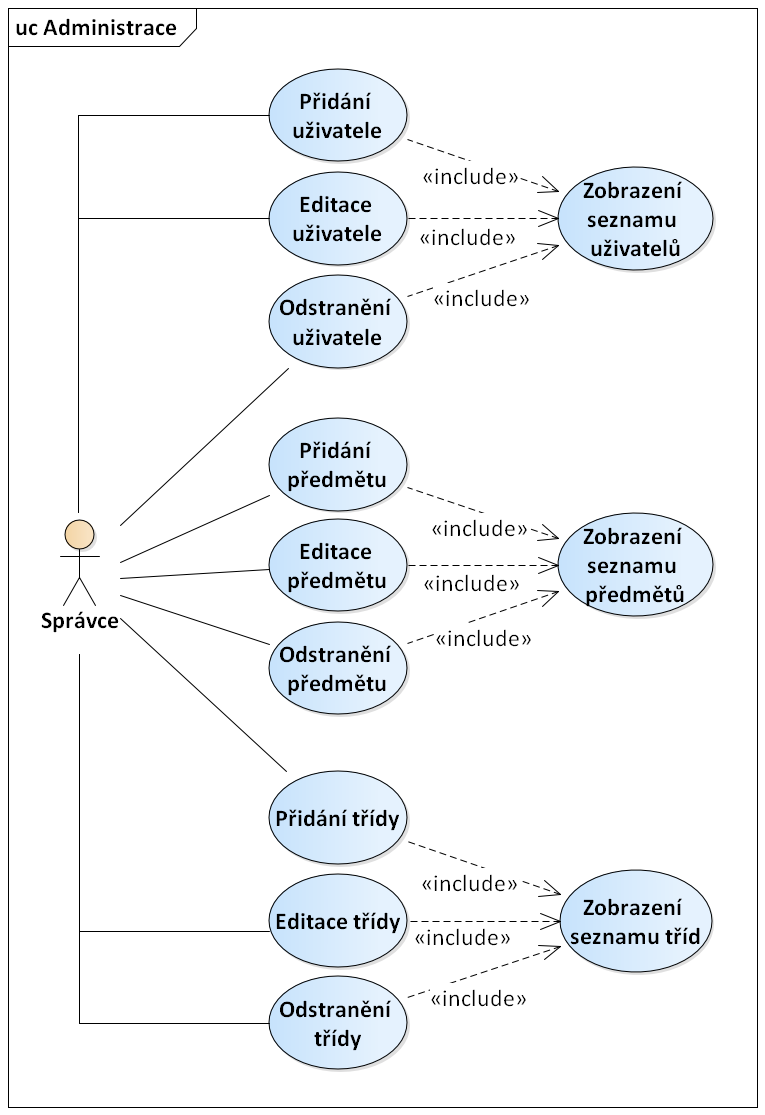
\includegraphics[width=0.80\textwidth]{images/administrace.png}
	\caption{Případy užití pro administraci systému}
	\label{pripady-administrace}
\end{figure}

\subsubsection*{UC14 Přidání uživatele}
Umožňuje správci přidat uživatele do systému. 
\begin{itemize}
    \item Správce se přepne do pohledu se seznamem uživatelů.
    \item Klikne na tlačítko pro přidání uživatele.
    \item Vyplní potřebné informace a potvrdí.
\end{itemize}

\subsubsection*{UC15 Editace uživatele}
Umožňuje správci editovat informace o uživateli.
\begin{itemize}
    \item Správce se přepne do pohledu se seznamem uživatelů.
    \item Klikne na tlačítko pro editaci uživatele.
    \item Změní potřebné informace a potvrdí.
\end{itemize}

\subsubsection*{UC16 Odebrání uživatele}
Umožňuje správci odebrat uživatele ze systému. 
\begin{itemize}
    \item Správce se přepne do pohledu se seznamem uživatelů.
    \item Klikne na tlačítko pro odebrání uživatele.
\end{itemize}

\subsubsection*{UC17 Přidání třídy}
Umožňuje správci přidat třídu do systému. 
\begin{itemize}
    \item Správce se přepne do pohledu se seznamem tříd.
    \item Klikne na tlačítko pro přidání třídy.
    \item Vyplní potřebné informace a potvrdí.
\end{itemize}

\subsubsection*{UC18 Editace třídy}
Umožňuje správci editovat informace o třídě.
\begin{itemize}
    \item Správce se přepne do pohledu se seznamem tříd.
    \item Klikne na tlačítko pro editaci třídy.
    \item Změní potřebné informace a potvrdí.
\end{itemize}

\subsubsection*{UC19 Odebrání třídy}
Umožňuje správci odebrat třídu ze systému. 
\begin{itemize}
    \item Správce se přepne do pohledu se seznamem tříd.
    \item Klikne na tlačítko pro odebrání třídy.
\end{itemize}

\subsubsection*{UC20 Přidání předmětu}
Umožňuje správci přidat předmět do systému. 
\begin{itemize}
    \item Správce se přepne do pohledu se seznamem předmětů.
    \item Klikne na tlačítko pro přidání předmětu.
    \item Vyplní potřebné informace a potvrdí.
\end{itemize}

\subsubsection*{UC21 Editace předmětu}
Umožňuje správci editovat informace o předmětu.
\begin{itemize}
    \item Správce se přepne do pohledu se seznamem předmětů.
    \item Klikne na tlačítko pro editaci předmětu.
    \item Změní potřebné informace a potvrdí.
\end{itemize}

\subsubsection*{UC22 Odebrání předmětu}
Umožňuje správci odebrat předmět ze systému. 
\begin{itemize}
    \item Správce se přepne do pohledu se seznamem předmětů.
    \item Klikne na tlačítko pro odebrání předmětu.
\end{itemize}

\subsubsection*{UC23 Zobrazení seznamu uživatelů}
Umožňuje správci zobrazit seznam uživatelů v systému. Systém umožňuje zobrazení tří skupin uživatelů:
\begin{itemize}
    \item žáků,
    \item rodičů, 
    \item zaměstnanců.
\end{itemize}

\subsubsection*{UC24 Zobrazení seznamu tříd}
Umožňuje správci zobrazit seznam tříd v systému.

\subsubsection*{UC25 Zobrazení seznamu předmětů}
Umožňuje správci zobrazit seznam předmětů v systému.

\section{Architektura}
Architektura informačního systému definuje strukturu systému. Ta se skládá z jednotlivých komponent, jejich vlastností a vztahů mezi nimi \cite{sw-architektura}. Pro tento informační systém bude zvolena třívrstvá architektura, která je vhodná pro složitější aplikace. Třívrstvá architektura rozděluje strukturu systému na tři vrstvy - prezentační, aplikační a datovou.

Prezentační vrstva slouží pro komunikaci s uživatelem. V této vrstvě budou uloženy CSHTML soubory, třídy zpracovávající požadavky od uživatelů, apod. Aplikační vrstva obsahuje business logiku systému. Zde budou probíhat jednotlivé procesy a výpočty. Datová vrstva zajišťuje persistenci dat, nejčastěji s pomocí databáze. V této vrstvě bude probíhat komunikace s databází a budou zde uloženy jednotlivé modely, které představují tabulky v databázi.

\subsection{Moduly}
Informační systém bude rozdělen na moduly podle funkčnosti. Rozdělení na moduly bude probíhat v každé vrstvě třívrstvé architektury a zajistí splnění nefunkčního požadavku N3, který požaduje snadnou rozšiřitelnost systému.

Na obrázku \ref{architektura} je zobrazen návrh architektury systému. Datová vrstva bude používat Entity Framework Core, který slouží k mapování objektů na relační data. Využíván bude v kombinaci s návrhovým vzorem repository. Každý modul bude mít své vlastní repository, které bude obsahovat dotazy do databáze.

V aplikační vrstvě budou všechny moduly rozděleny do vlastních funkčních celků, ve kterých budou probíhat procesy a funkcionalita spojená s daným modulem. 

Co se prezentační vrstvy týče, každý modul bude používat návrhový vzor MVC (model-view-controller), který řeší problémy prezentační vrstvy. Návrhový vzor MVC rozděluje strukturu kódu na tři vrstvy -- modely, views (pohledy) a controllers (kontrolery).

Model je nejnižší vrstva tohoto vzoru. Je tvořen doménovými objekty a reprezentuje data aplikace. Pomocí těchto objektů se předávají data do pohledů a z pohledů do kontrolerů. Pohledy se starají o uživatelské rozhraní. Tato vrstva se skládá z HTML šablon,  do kterých lze vkládat data z kontrolerů. V šablonách lze kombinovat čisté HTML s server-side kódem. Kontrolery se starají o zpracovávání uživatelských požadavků z pohledů. Každý požadavek je pomocí routování mapován na určitou akci v kontroleru. Zjednodušeně lze říci, že kontrolery řídí celkový průchod aplikací. \cite{dp-mvc} 
\clearpage

\begin{figure}[h]
	\centering
	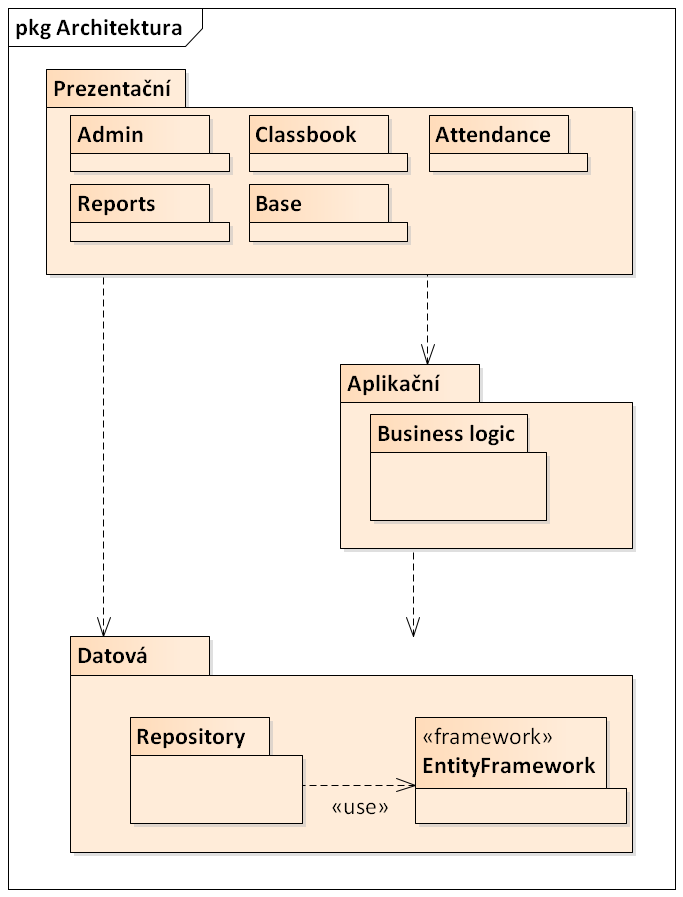
\includegraphics[width=0.8\textwidth]{images/architektura.png}
	\caption{Třívrstvá architektura - relaxovaná}
	\label{architektura}
\end{figure}

Informační systém je rozdělen na následujících pět modulů.

\subsubsection*{Modul administrace - Admin}
Modul administrace slouží pro správu systému. Tento modul zajistí splnění funkčního požadavku F2. Do této sekce bude mít přístup pouze uživatel s rolí správce. Bude zde probíhat správa uživatelů, tříd a předmětů.

\subsubsection*{Modul třídní knihy - Classbook}
V tomto modulu bude probíhat práce s třídní knihou. Tento modul bude pokrývat funkční požadavky F3, F5 a F7. Do této sekce budou mít přístup všichni uživatelé s rolí učitel, třídní učitel, zástupce ředitele, ředitel a správce. Budou zde probíhat zápisy do třídních knih, vytváření událostí v hodinách a exporty třídních knih.

\subsubsection*{Modul docházka - Attendance}
Zde bude probíhat veškerá práce s omluvenkami. Modul docházka zajistí pokrytí funkčního požadavku F4. Modul bude dostupný uživatelům s rolí rodič a třídní učitel. Rodič zde bude vytvářet omluvenky a odesílat je třídnímu učiteli. Třídní učitel bude v tomto modulu omlouvat absenci žáka na základě omluvenek od rodiče.

\subsubsection*{Modul přehledy - Reports}
Pomocí tohoto modulu budou zobrazovány přehledy o žácích, čímž se splní funkční požadavek F6. Zde budou mít přístup všichni přihlášení uživatelé. Uživatelům z řad zaměstnanců budou poskytnuty přehledy o všech žácích. Rodičům, respektive žákům budou zobrazeny přehledy pouze o potomcích, respektive o sobě.

\subsubsection*{Základní modul - Base}
V základním modulu budou probíhat obecné funkcionality, například autentizace a autorizace. Tento modul splní funkční požadavek F1. Jelikož se v tomto modulu budou vyskytovat pouze obecné funkcionality, bude přístupný všem uživatelům.


\section{Návrh obrazovek}
V této části bude navrhnuto uživatelské rozhraní několika hlavních obrazovek. Vždy bude navržena pouze základní kostra obrazovky, finální design aplikace bude vyřešen až při její implementaci.

Základní kostra bude navržena pro obrazovku, kde probíhá zápis do třídní knihy, pro obrazovku, kde třídní učitel schvaluje omluvenky a pro úvodní stránku rodičovského portálu.
\clearpage

Na obrázku \ref{obrazovka-zapis} je zobrazena obrazovka pro zápis do třídní knihy. Lze vidět, že zápis se vztahuje k vybranému datu. To lze vybrat po rozkliknutí kalendáře. Defaultně se vyplňuje aktuální datum. Zápis se vytváří pomocí tlačítka pro nový zápis, které přesměruje uživatele na formulář, kde se vyplní předmět a téma. Absence se vyplní ve formuláři, který se vyvolá stisknutím tlačítka \uv{Absence}. Případné události se vyberou ze seznamu po stisknutí tlačítka \uv{Další}.

\begin{figure}[h]
	\centering
	\frame{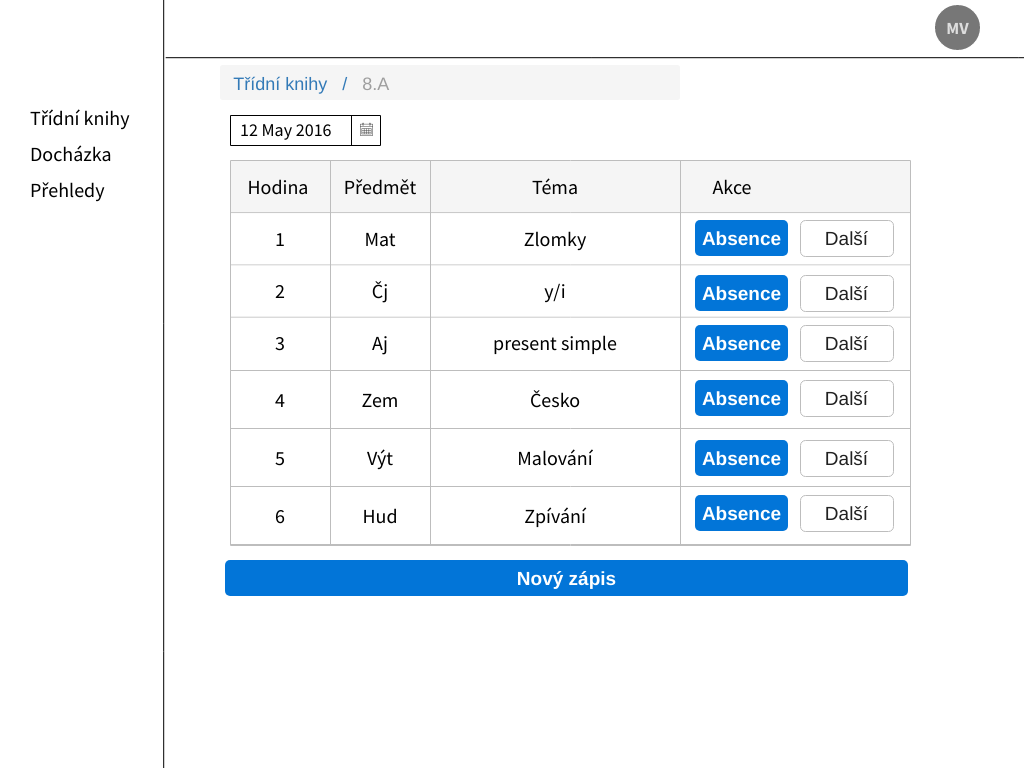
\includegraphics[width=\textwidth]{images/obrazovka_zapis.png}}
	\caption{Obrazovka pro zápis do třídní knihy}
	\label{obrazovka-zapis}
\end{figure}

Na obrázku \ref{obrazovka-omluvenky} lze vidět obrazovku, kde třídní učitel schvaluje omluvenky. Třídní učitel vidí seznam omluvenek, které může potvrdit či zamítnout. Může si také zobrazit detail, kde uvidí, pro které absence je omluvenka napsána.
\clearpage

\begin{figure}[h]
	\centering
	\frame{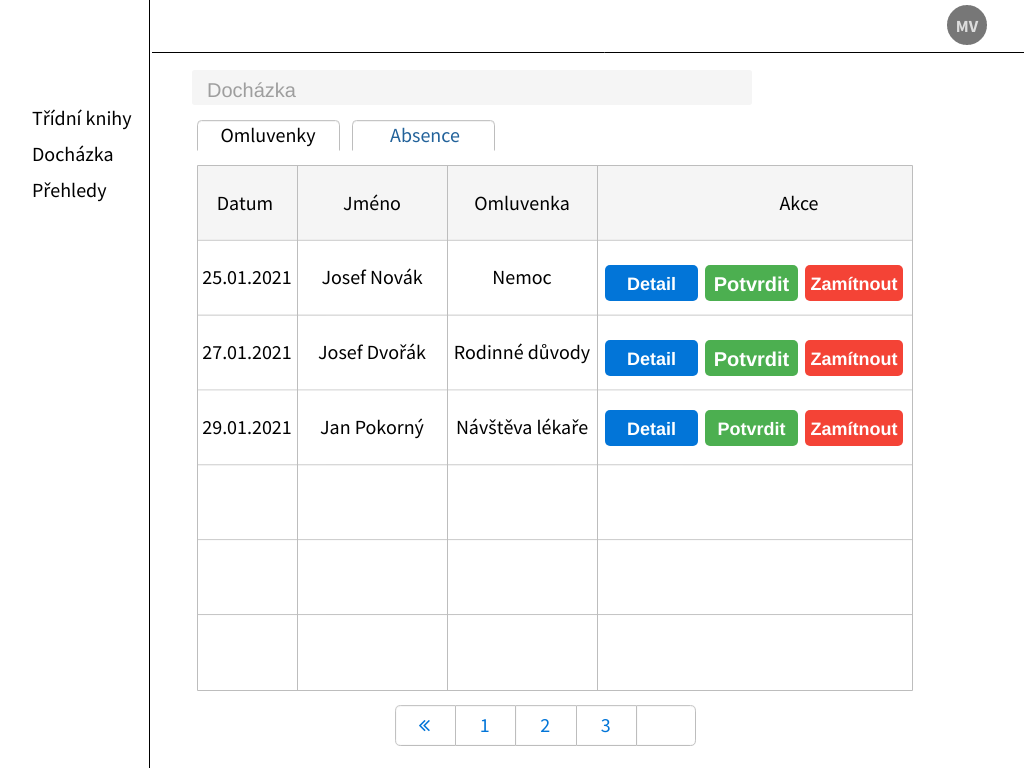
\includegraphics[width=\textwidth]{images/obrazovka_omluvenky.png}}
	\caption{Obrazovka pro schvalování omluvenek}
	\label{obrazovka-omluvenky}
\end{figure}

Obrázek \ref{obrazovka-rodic} zobrazuje návrh rodičovského portálu. Rodič vidí seznam svých dětí a rychlý přehled o nových informacích. Detaily o těchto informacích si rodič může zjistit v příslušných přehledech. Do nich se přepne pomocí navigačního menu vlevo stránky.
\clearpage

\begin{figure}[H]
	\centering
	\frame{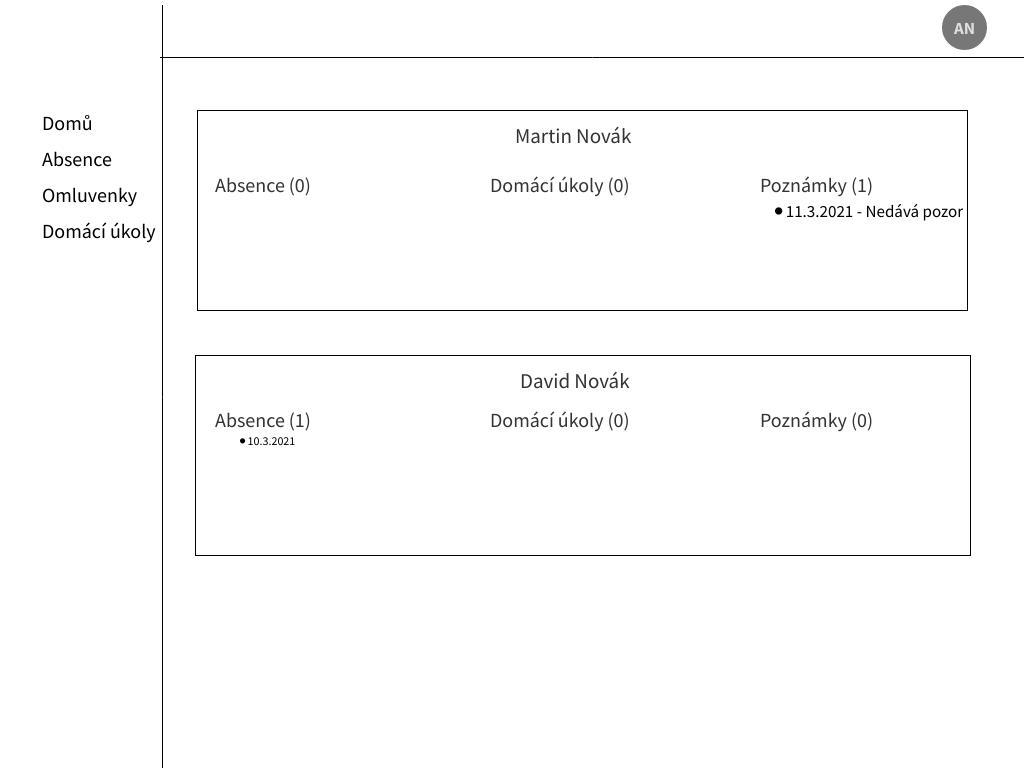
\includegraphics[width=\textwidth]{images/obrazovka_rodic.png}}
	\caption{Prostředí pro rodiče}
	\label{obrazovka-rodic}
\end{figure}


